\documentclass{article}

\usepackage[english]{babel}

\usepackage[letterpaper,top=2cm,bottom=2cm,left=3cm,right=3cm,marginparwidth=1.75cm]{geometry}

% Useful packages
\usepackage{amsmath}
\usepackage{graphicx}
\usepackage[colorlinks=true, allcolors=blue]{hyperref}
\usepackage{listings}
\usepackage[T1]{fontenc}
\usepackage{tgbonum}
\usepackage{textcomp}
\usepackage{setspace}
\usepackage{subcaption}

\lstdefinestyle{bashStyle}{
  showstringspaces=false,
  language=bash,
  basicstyle=\small\sffamily,
  frame=tb,
  columns=fullflexible,
  linewidth=\linewidth,
  xleftmargin=0.075\linewidth,
  breaklines=true,
  literate =
    {'}{{\textquotesingle}}1
    {-}{{-}}1
}

\title{Modul 2 - Using S3 to store data from IoT core}
\author{}

\begin{document}
\lstset{language=Bash,upquote=true}
\begin{minipage}{0.2\textwidth}
  
\includegraphics[width=\linewidth]{assets/logo_lks.png}
\end{minipage}
\hfill%
\begin{minipage}{0.75\textwidth}
  {\fontfamily{cmr}\selectfont
    {\huge
    \textbf{LOMBA KOMPETENSI SISWA (LKS)}
    \vspace{4mm} 
    \textbf{SEKOLAH MENENGAH KEJURUAN}
    \vspace{4mm} 
    \textbf{TINGKAT PROVINSI JAWA BARAT}
    \vspace{4mm} 
    \textbf{TAHUN 2024}
    }
  }
\end{minipage}
\vspace{30mm} %5mm vertical space
\begin{center}
  {\fontfamily{cmr}\selectfont
    {\huge
      \textbf{NASKAH SOAL}\\
      \vspace{10mm} 
      \textbf{Bidang Lomba}\\
      \vspace{4mm} 
      \textbf{Cloud Computing}
    }
  }
\end{center}
{\let\newpage\relax\maketitle}

\vspace{10mm} 

\begin{minipage}{.33\textwidth}
  \centering
    
\includegraphics{assets/disdik_jabar.png}
\end{minipage}
\begin{minipage}{.33\textwidth}
  \centering
    
\includegraphics{assets/smk.jpg}
\end{minipage}
\begin{minipage}{.33\textwidth}
  \centering
    
\includegraphics{assets/merdeka_belajar.png}
\end{minipage}

\vspace{10mm} 

\begin{minipage}{0.2\textwidth}
  
\includegraphics[width=\linewidth]{assets/disdik_jabar_logo.png}
\end{minipage}
\hfill%
\begin{minipage}{0.75\textwidth}
  \centering
  {\fontfamily{lmss}\selectfont
    {\large
    \textbf{PEMERINTAH DAERAH PROVINSI JAWA BARAT}\\
    }
    {\Large
    \textbf{DINAS PENDIDIKAN}\\
    }
  }
    \vspace{2mm} 
    Jalan Dr. Radjiman No. 6 Telp. (022) 4264813 Fax. (022) 4264881\\
    Website: disdik.jabarprov.go.id\\
    Email: disdik@jabarprov.go.id/sekretariatdisdikjabar@gmail.com\\
    BANDUNG - 40171
\end{minipage}
\newpage

\begin{figure*}[h]
\centering
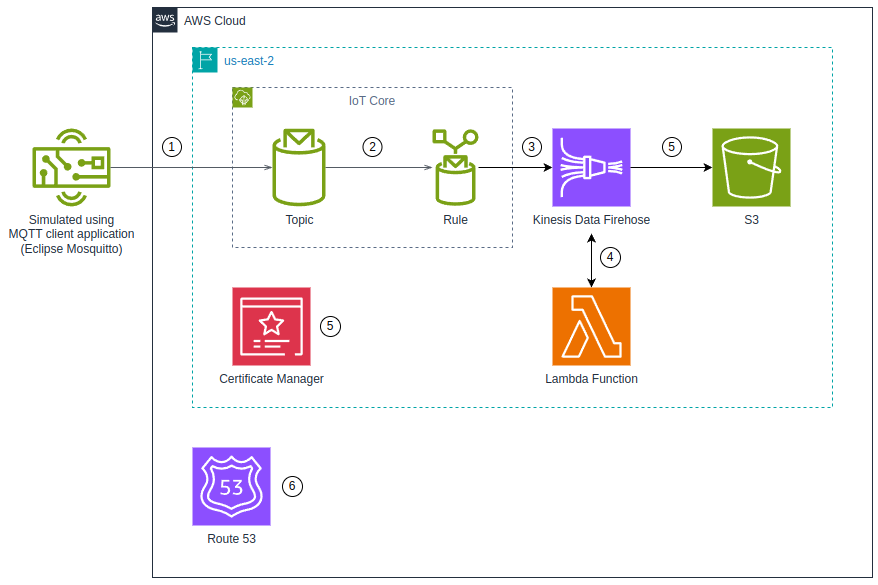
\includegraphics[width=\textwidth]{assets/architecture.png}
\caption{\label{fig:architecture}Architecture Diagram}
\end{figure*}

\section{Overview}
Storing raw IoT data may incur significant expenses due to the sheer volume of the data involved.
S3 offers a cost-effective solution for storing data, especially when dealing with large datasets. It follows a pay-as-you-go pricing model, meaning you only pay for the storage you use, without any upfront costs or long-term commitments.
Your task is to build a solution to efficiently store raw data from IoT core to S3 using Kinesis Firehose. Additional preprocessing such as using Glue, Athena dan QuickSight is beyond the scope of this task.

\section{General Rules}
\begin{enumerate}
    \item Failure to comply with the rules will result in immediate disqualification.
    \item You have 3 hours to finish the tasks.
    \item You may not open any website unless otherwise specified in section \ref{references} and you may open the control panel of your domain provider to update the nameserver to Route 53.
    \item Using the search feature from the AWS documentation website is allowed. However opening other AWS website such as AWS Solutions Library is NOT permitted. If you are unsure about the eligibility of the site you want to open, please ask.
    \item You may use AWS Console and AWS CLI to deploy the solutions. You may not use SAM, CloudFormation, or CDK.
    \item During the event, multiple login is not permitted.
    \item If you have any question, do not hesitate to ask.
\end{enumerate}

\section{Architecture}\label{architecture}

Refer to Figure \ref{fig:architecture}.
\begin{enumerate}
  \item The MQTT software stream payloads to the AWS IoT Core message broker to a specific MQTT topic.
  \item The AWS IoT rule activates upon detecting a payload within its designated topic. The rule is configured with an Amazon Kinesis Data Firehose action. 
  \item Amazon Kinesis Data Firehose buffers the incoming payloads, then it will deliver them to the data store once either size or time thresholds are met, whichever comes first.
  \item Before delivering to the destination, Kinesis Data Firehose execute an AWS Lambda function to transform the payloads in batches. In this case, the lambda function will add and attributed named "processedAt" with current timestamp as the value and then return the modified payload to Kinesis Data Firehose.
  \item The modified payloads are compressed and put into an Amazon S3 bucket.
  \item Certificate Manager is used to provide certificate for IoT Core's custom domain.
  \item Route 53 is used to point the custom domain to IoT Core's endpoint.
\end{enumerate}

\section{Information}\label{information}

\begin{enumerate}
  \item The repository URL for the required source code to deploy this solution is:\\
  \href{https://github.com/kensasongko/lksccjabar2024modul3_aplikasi}{https://github.com/kensasongko/lksccjabar2024modul3\_aplikasi}
  \item This solution must be deployed in \textbf{us-east-2 (Ohio)} region. Deploying in another region will result in a major point reduction.
  \item An automated scoring system will check your AWS account to calculate the score of your task.
  \item In order check your progress, the scoring system needs an AWS credential with administrator privilege. You will be asked to provide the AWS credential.
  \item AWS tag is used by the scoring system to find your solution. Forgetting to add the required tag or adding the same tag value to multiple instance may result in an unexpected behavior and thus lower your score.
  \item The system will calculate 90\% of the final score. The remaining 10\% will be evaluated by checking manually in front of the participants.
  \item If multiple participants complete the assignment, their completion times will factor into the manual scoring process. For instance, the first participant to finish will receive a full score, while subsequent finishers will incur minor penalties.
  \item Mosquitto MQTT client is used as an example to test the deployment.
\end{enumerate}

\section{Task}
Your task is to create the solution from the section \ref{architecture}.
\begin{enumerate}
\item Create an S3 bucket with the following configuration:
  \begin{itemize}
    \item Block all public access.
    \item Bucket Versioning: Disable
    \item Tag: Key=LKS-CC-2024, Value=LKS-IOT-S3
  \end{itemize}
\item Deploy Lambda.
  \begin{itemize}
    \item The source code of the lambda function can be found in section \ref{information}.
    \item Create and deploy the lambda function with the following configuration:
    \begin{itemize}
      \item Lambda runtime: python3.12
      \item Timeout: 1 minutes
      \item Memory size: 256 MB
      \item Ephemeral storage: 512 MB
      \item Architecture: arm64
      \item Tag: Key=LKS-CC-2024, Value=LKS-IOT-LAMBDA
    \end{itemize}
  \end{itemize}
\item Create Kinesis Data Firehose with the following configuration:
  \begin{itemize}
    \item Source: Direct PUT
    \item Destination: S3
    \item Enable transform source records with AWS Lambda:
    \begin{itemize}
      \item Choose the Lambda function you have previously deployed.
      \item Version or alias: \$LATEST
      \item Buffer size: 1 MB
      \item Buffer interval: 60 seconds
    \end{itemize}
    \item New line delimiter: Enabled
    \item S3 bucket prefix: data/
    \item S3 bucket error output prefix: error/
    \item S3 bucket and S3 error output prefix time zone: UTC
    \item S3 buffer hints:
    \begin{itemize}
      \item Buffer size: 1 MB
      \item Buffer interval: 60 seconds
    \end{itemize}
    \item Compression for data records: GZIP
    \item Tag: Key=LKS-CC-2024, Value=LKS-IOT-FIREHOSE
  \end{itemize}
\item Create an IoT Rule.
  \begin{itemize}
    \item Rule name: ToFirehose
    \item SQL version: 2016-03-23
    \item SQL statement: SELECT * \lstinline{FROM 'location/#'}
    \item Rule action: Amazon Data Firehose stream
    \item Amazon Data Firehose stream: The stream you have previously created
    \item Separator: \lstinline{\n}
    \item Batch mode: Enabled
    \item IAM Role: Create new role named IoTRuleToFirehoseRole
    \item Tag: Key=LKS-CC-2024, Value=LKS-IOT-RULE
  \end{itemize}
\item Create IoT Policy with the following configuration:
  \begin{itemize}
    \item Allow iot:Connect to *
    \item Allow iot:Publish to *
    \item Tag: Key=LKS-CC-2024, Value=LKS-IOT-POLICY
  \end{itemize}
\item Create IoT certificate with the following configuration:
  \begin{itemize}
    \item Auto-generate new certificate.
    \item Attach the IoT Policy you have created.
  \end{itemize}
\item Create a CNAME record in Route 53 named lks-iot from your domain with your IoT Core device data endpoint as the value of the record.
\item Request a public certificate for *.[YOUR\_DOMAIN] from AWS Certificate Manager and validate the certificate using DNS validation.
\item Create IoT domain configurations with the following configuration:
  \begin{itemize}
    \item Name: lks-iot
    \item Domain type: Customer managed domain
    \item Domain name: lks-iot.[YOUR\_DOMAIN]
    \item Server certificate: Choose the certificate you have previously requested in ACM.
  \end{itemize}
\end{enumerate}
\section{How to test your deployment}
\begin{enumerate}
  \item Using the IoT certificate you have downloaded, execute the following command on your terminal:
    \begin{lstlisting}
mosquitto_pub -h lks-iot.[YOUR_DOMAIN] -p 8883 \
  --key /path/to/xxx.private.pem.key \
  --cert /path/to/xxx.certificate.pem.crt \
  --cafile /path/to/AmazonRootCA1.pem \
  -t location/device1 -m '{"hello":"test"}' -i d1 -d
    \end{lstlisting}
    The output should be similar to:
    \begin{lstlisting}
Client d1 sending CONNECT
Client d1 received CONNACK (0)
Client d1 sending PUBLISH (d0, q0, r0, m1, 'location/d1', .(9 bytes))
Client d1 sending DISCONNECT
    \end{lstlisting}
  \item Check your S3 bucket, ensure the bucket contains your payload along with processedAt attribute.
  For example:
  \begin{lstlisting}
  {"hello": "test", "processedAt": "2024-05-05 03:57:41"}
  \end{lstlisting}
\end{enumerate}
\section{References}\label{references}
\begin{itemize}
  \item \href{https://mosquitto.org/}{Eclipse Mostquitto}
  \item \href{https://docs.aws.amazon.com/iot/latest/developerguide/what-is-aws-iot.html}{AWS IoT Core}
  \item \href{https://docs.aws.amazon.com/firehose/latest/dev/what-is-this-service.html}{Amazon Data Firehose}
  \item \href{https://docs.aws.amazon.com/lambda/latest/dg/welcome.html}{AWS Lambda}
  \item \href{https://docs.aws.amazon.com/AmazonS3/latest/userguide/Welcome.html}{Amazon S3}
  \item \href{https://docs.aws.amazon.com/Route53/latest/DeveloperGuide/Welcome.html}{Amazon Route 53}
  \item \href{https://docs.aws.amazon.com/acm/latest/userguide/acm-overview.html}{AWS Certificate Manager}
\end{itemize}
\section*{Good luck!}

\begin{equation}
cos(\theta) = \frac{\vec{A}\cdot\vec{B}}{\lVert \vec{A} \rVert \cdot \lVert \vec{B} \rVert} = \frac{\sum_{i=1}^{n}A_i B_i}{\sqrt{\sum_{i=1}^{n}A_i^2} \sqrt{\sum_{i=1}^{n}B_i^2}}
\end{equation}

\begin{equation}
  KernelKMeansDistance(K_{ii}, K) = K_{ii} - \frac{2 * \sum_{x_j \in \pi_{c}} \alpha_{j} K_{ij}}{\sum_{x_j \in \pi_{c}} \alpha_{j}} + \frac{\sum_{x_j,x_l \in \pi_{c}} \alpha_{j} \alpha_{l} K_{jl}}{(\sum_{x{j}\in \pi_{c}} \alpha_{j})^2}
\end{equation}
\end{document}
